\documentclass[11pt,largemargins]{homework}

\newcommand{\hwname}{Giulio Nenna}
\newcommand{\hwemail}{s245717@studenti.polito.it}
\newcommand{\hwtype}{Homework}
\newcommand{\hwnum}{1}
\newcommand{\hwclass}{}
\newcommand{\hwlecture}{}
\newcommand{\hwsection}{}

% This is just used to generate filler content. You don't need it in an actual
% homework!
\usepackage{lipsum}
\usepackage{amssymb}
\usepackage[utf8]{inputenc}
\usepackage[T1]{fontenc}
\usepackage{lmodern}
\usepackage{amsfonts}
\usepackage{hyperref}
\usepackage{bbm}
\usepackage{amsmath}

\begin{document}
\maketitle

\question

  \begin{figure}[htb]\centering
    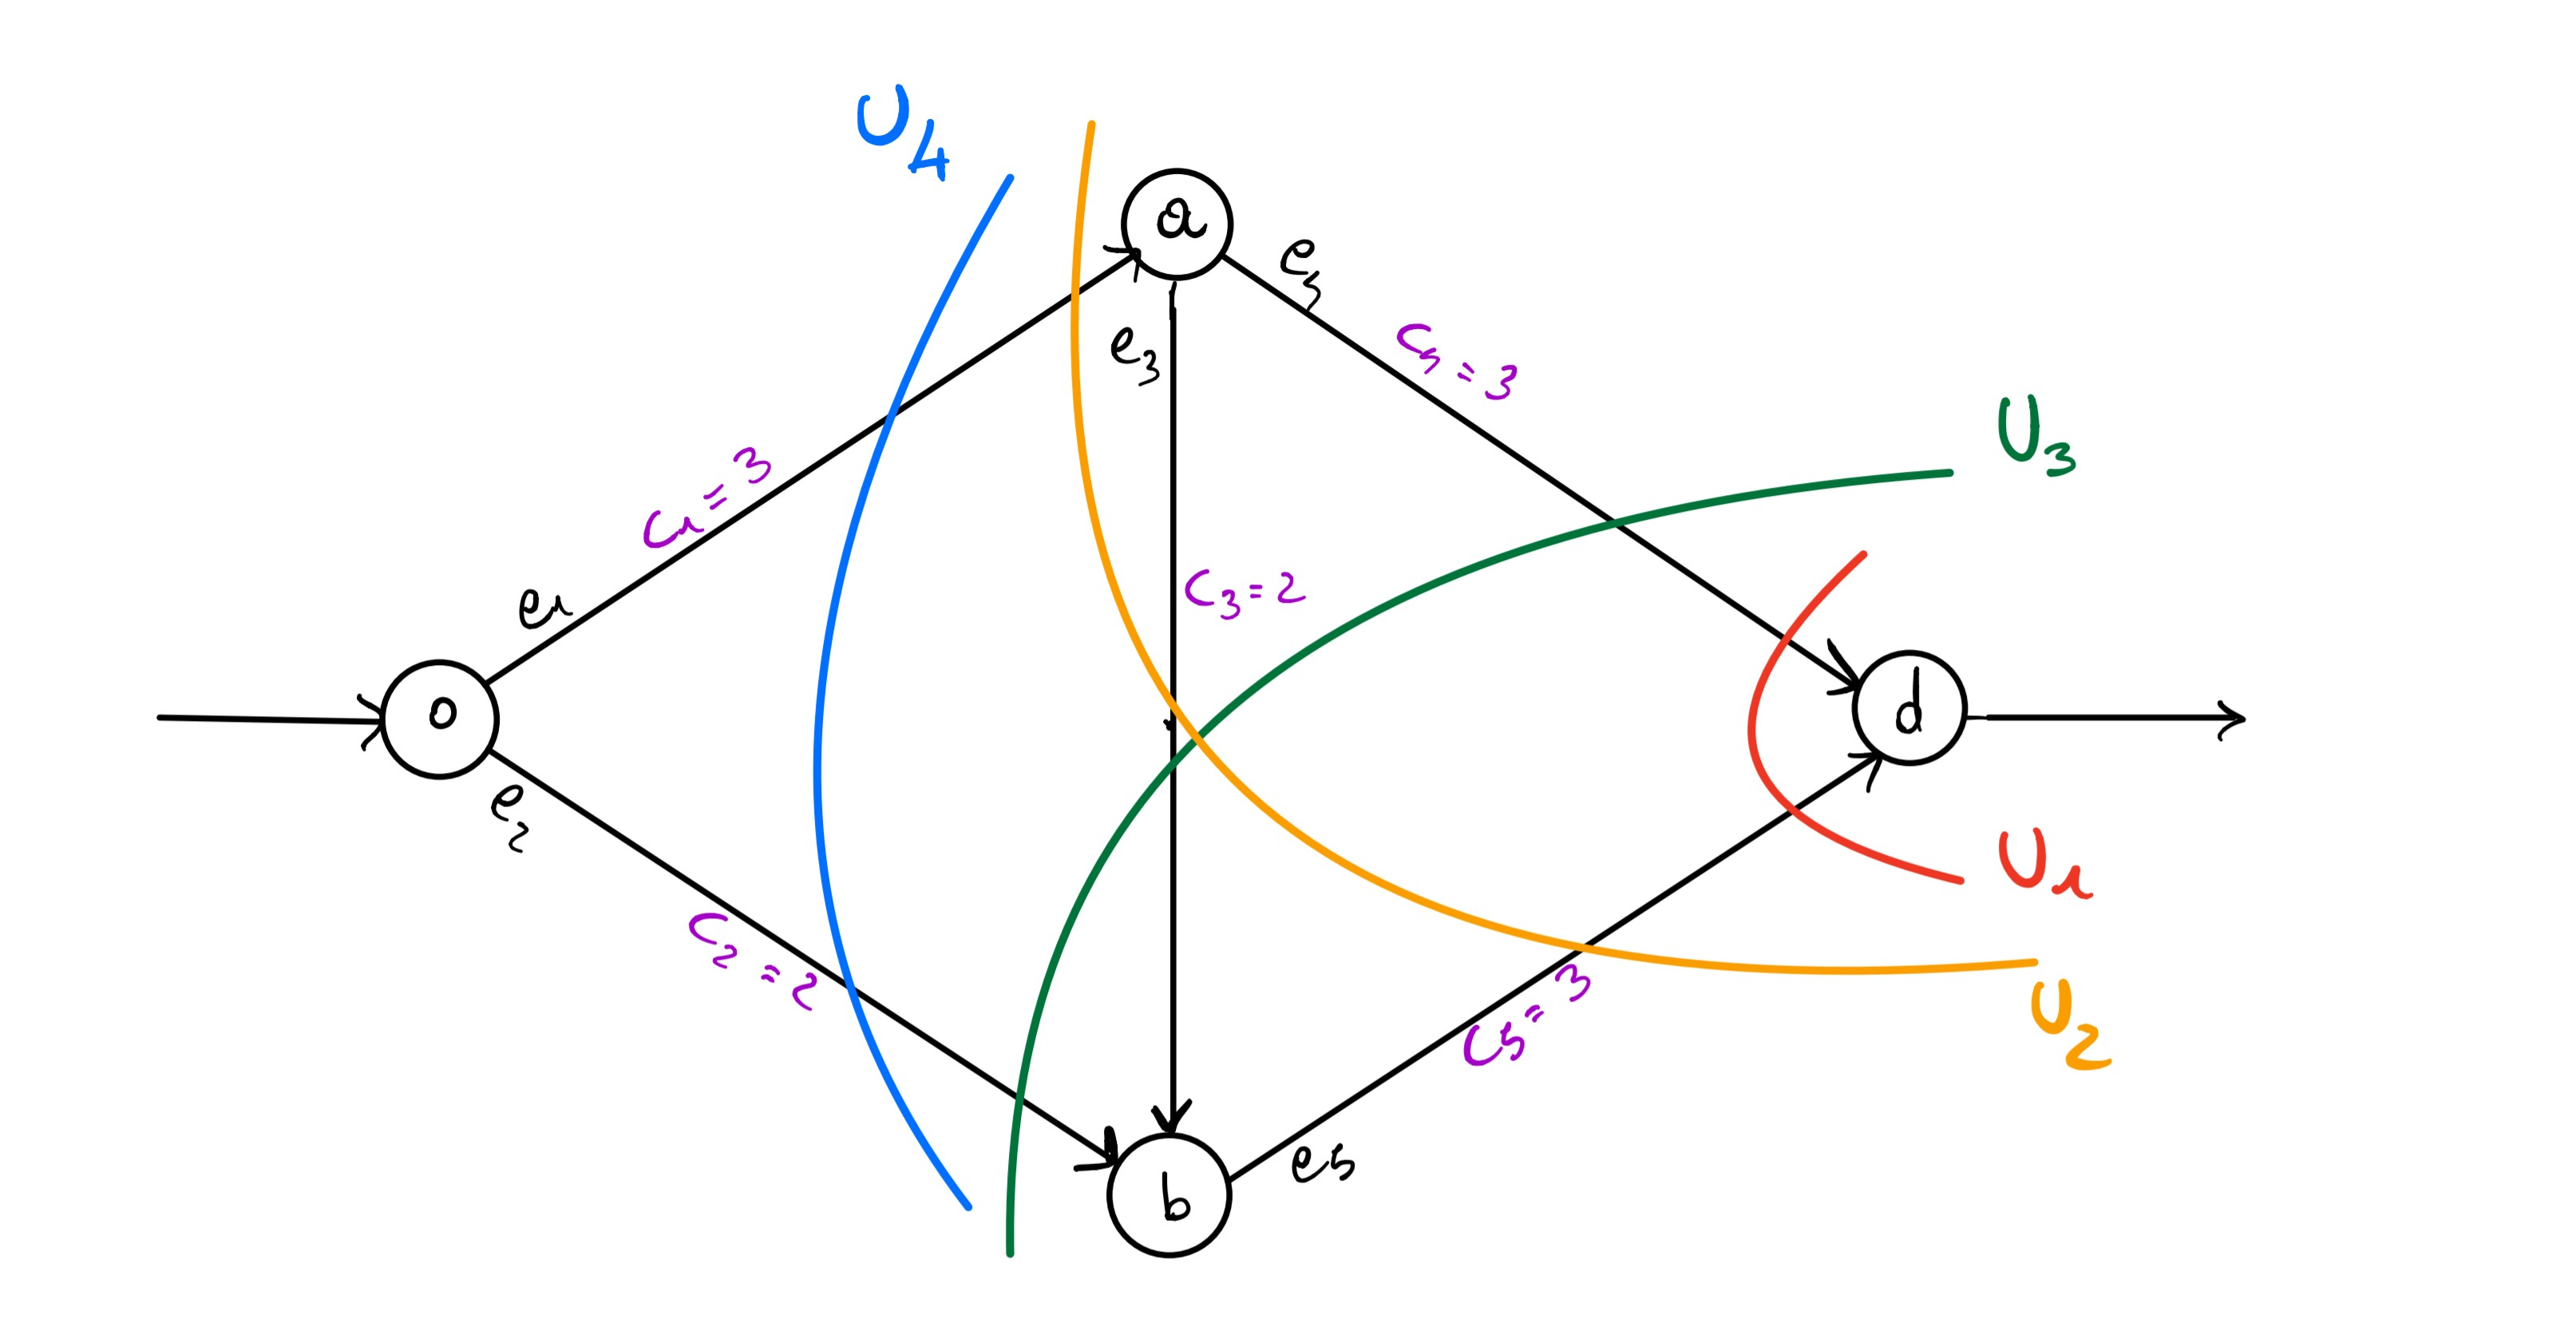
\includegraphics[scale=0.17]{ES1_Fig1.jpg}
  \end{figure}
  Tutti i possibili path \(o-d\) sono i seguenti:

  \begin{description}
    \item[1.] \(p_{(1)}= o -a-d\)
    \item[2.] \(p_{(2)}=o-b-d\) 
    \item[3.] \(p_{(3)}= o-a-b-d\) 
  \end{description}

  I possibili cut e annesse capacità sono:

  \begin{align*}
    U_1 = \{d\}\  && C(U_1)=5 \\
    U_2 = \{a, d\} && C(U_2)=5 \\
    U_3 = \{b,d\} && C(U_3)=7 \\
    U_4 = \{a,b,d\} && C(U_4)=5
  \end{align*}
  
  \begin{alphaparts}
    \questionpart
    Tutti i possibili colli di bottiglia del grafo hanno capacità pari a 5, quindi per ostruire qualsiasi tipo di flow unitario da \(o\) a \(d\) bisogna eliminare una capacità \(C^*\) tale che
    \begin{equation*}
      C^*<4
    \end{equation*}

    \questionpart
    Dal momento che vale il teorema del \textit{Max Flow - Min Cut}, le due unità di capacità devono essere distribuite in modo tale da capacità del minimo taglio. Poiché ci sono ben tre tagli su 4 che rappresentano un minimo taglio \((U_1, U_2, U_4)\) è necessario aumentare la capacità su archi in comune a questi tre tagli.\\
    Una scelta possibile potrebbe essere quella di aggiungere un'unità di capacità ciascuno agli archi \(e_1\) ed \(e_4\) in modo tale che i tagli risultino:
    
  \begin{align*}
    U_1 = \{d\}\  && C(U_1)=6 \\
    U_2 = \{a, d\} && C(U_2)=6 \\
    U_3 = \{b,d\} && C(U_3)=9 \\
    U_4 = \{a,b,d\} && C(U_4)=6
  \end{align*}

  Aumentando in questo modo il massimo troughput da 5 a 6

  \end{alphaparts}

\question
  This question's number will be auto-incremented.

  \lipsum[2]

\question*{Super Fancy Named Question}
  This question was given a fancy name!

  \lipsum[3]

% Sometimes questions get separated from their bodies. Use a \newpage to force
% them to wrap to the next page.
\newpage
\question
  Using the \texttt{induction} environment is a great way to typeset induction proofs!
  \begin{induction}
    \basecase
      Here I have my base case.
      This is usually about 1-2 lines of text that is not entirely difficult to come up with.
      That doesn't mean it's not important though!
    \indhyp
      Assume cool things to make proof work. Look, math:
      \[a^2 + b^2 = c^2\]
    \indstep
      Prove all the things.  When in doubt, write in Latin, because things
      written in Latin sound more true.  Lorem ipsum dolor sit amet, consectetur
      adipiscing elit. Maecenas tempor risus in dapibus aliquam. Donec at
      euismod dui. In libero turpis, blandit quis vestibulum ac, rutrum sit amet
      est. Suspendisse nec lacus vel dui lobortis lacinia at sit amet risus.
      Fusce dui ex, imperdiet nec finibus ut, bibendum a lacus.
  \end{induction}

  Therefore, we have proven the claim by induction in the \texttt{induction} environment.

\question
  Use the arabicparts environment to include the questionCounter number in the list.
  \begin{arabicparts}
    \questionpart Use \LaTeX
    \questionpart ???
    \questionpart Profit!
  \end{arabicparts}

  \lipsum[7]

\question
  Use the alphaparts environment for letters instead of numbers.
  \begin{alphaparts}
    \questionpart
      Use \LaTeX
    \questionpart ???
    \questionpart Profit!
  \end{alphaparts}

\question
    Question part numbers are auto-incremented within the same question, so if you have some question parts...

    \begin{alphaparts}
        \questionpart
            Use \LaTeX
        \questionpart ???
    \end{alphaparts}

    Followed by some additional text, followed by some more question parts:

    \begin{alphaparts}
        \questionpart Profit!
    \end{alphaparts}

    All parts will be continuously numbered.

\question
  Question numbers continue to auto-increment, regardless of question type.

  \lipsum[4]

% Use \renewcommand{\questiontype}{<text>} to change what word is displayed
% before numbered questions
\renewcommand{\questiontype}{Task}
\question
  This question has a different question type!

  \lipsum[5]

\renewcommand{\questiontype}{Question}

\question
  You can still do things like nesting lists inside of these environments.
  \begin{alphaparts}
    \questionpart Use \LaTeX
      \begin{enumerate}
        \item Open terminal
        \item Open vim
        \item Write LaTeX
      \end{enumerate}
    \questionpart ???
    \questionpart Profit!
  \end{alphaparts}

  \lipsum[9]

% Use the \setcounter{questionCounter}{<x>} to force the question number to a
% particular question. If your written homework's question start at number 9001,
% use the following
\setcounter{questionCounter}{9000}
\question
  \href{https://www.youtube.com/watch?v=SiMHTK15Pik}{It's over 9000!!!}

  \lipsum[6]


\section{}
  You can also use the \texttt{section} macro for starting a question.

  \lipsum[10]

\section*{Using the \texttt{section} Macro}
  The starred \texttt{section*} works as well.

  \lipsum[11]

\end{document}
